Options to collect consent are minimal (also see previously noted restriction on providing URLs). However, respondents can break off the survey at all times, and this is identified at each point of the survey. When first offered the survey, all respondents are offered the first question of the questionnaire, without an introduction (unless the researcher explicitly makes the first question into an introduction or invitation, though this is not usually done). At this time, respondents can choose to answer the question, choose to see a different question, or choose to skip the survey. 
% what happens if a respondent clicks "skip survey" once­ will they get solicited again on a different platform, or does Google Consumer Surveys recognize that the individual does not want to answer those specific questions, and won't ask again for a few weeks/months/ever?
It is not obvious from the information provided by Google what happens when a respondent clicks "skip survey" - does a cookie get set that prevents the respondent from ever seeing this particular survey again, or is there potential for presenting the question to the respondent again, on any of the platforms on which \ac{GCS} presents surveys? Note however that there does not seem to be  limit to the number of times a respondent can skip a question or a survey. 

A link to information about Google Consumer Surveys (but not the researcher) and Google's Privacy policy are prominently displayed. This setup cannot be changed. Figure~\ref{fig:anatomy} shows an example. 
\begin{figure}
	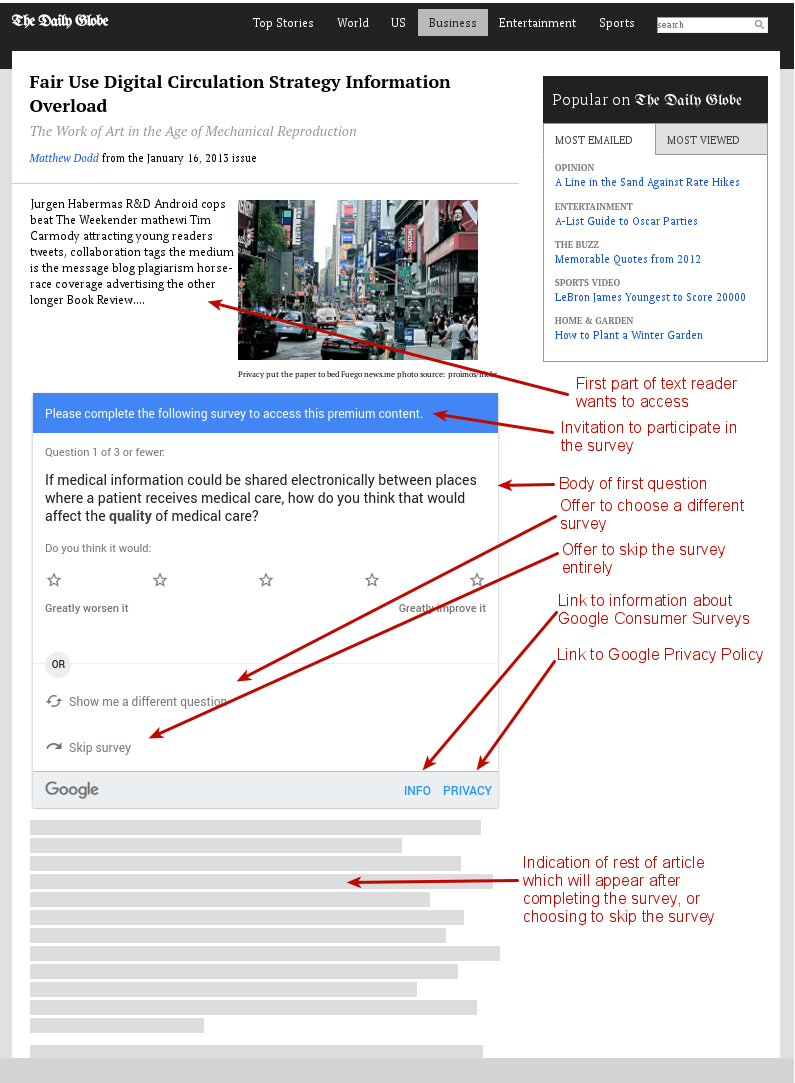
\includegraphics[width=\textwidth]{Selection_359.png}
	\caption{\label{fig:anatomy}Anatomy of a page}
\end{figure}
The same generic setup repeats for each question. After answering the last question, or skipping the survey, the desired article appears. Thus, at all times, all respondents have a way to skip a shown question and still access the premium content.

\cite{doi:10.1093/pan/mpw016} note that non-conforming content can be embedded into the questionnaire using images, however, this cannot be used for all question types.

\subsubsection{Privacy and Confidentiality}
All personal identifiers are removed from the data by \ac{GCS}, or never collected. All quasi-identifiers are estimated or imputed. No member of the research team will ever have access to any personal identifiers, as this information is never provided to purchasers of survey data. 